
\documentclass[tikz, border=10pt]{standalone}
\usepackage{tikz}
\usepackage{graphicx}
\usetikzlibrary{positioning, shadows, calc, shapes}

\begin{document}
\section{MLP-Mixer Architecture}
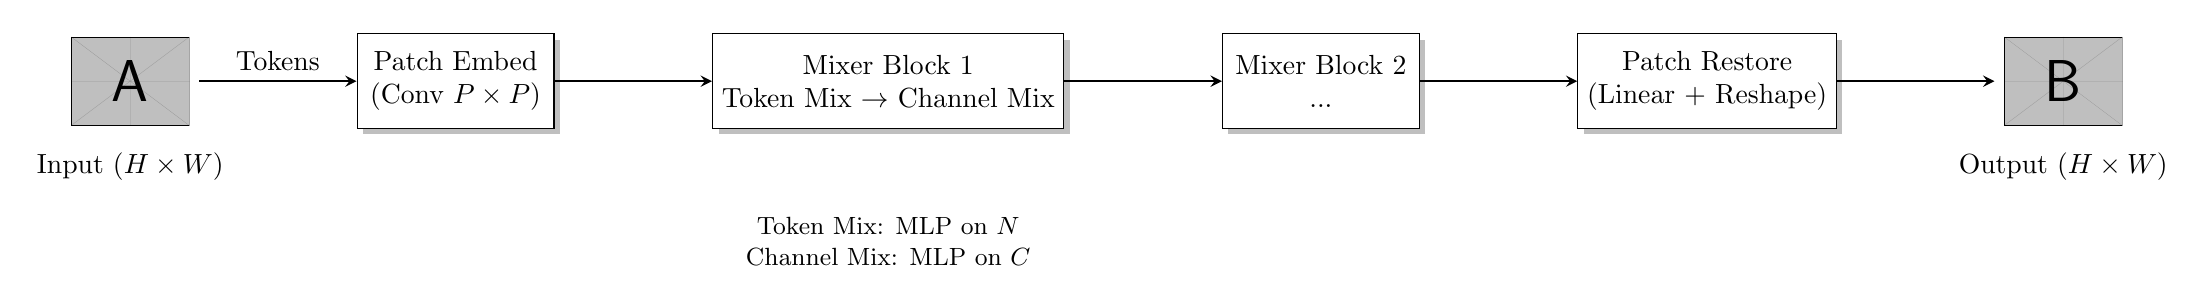
\begin{tikzpicture}[
    node distance=1.5cm,
    block/.style={draw, rectangle, minimum height=1.2cm, minimum width=2.5cm, align=center, fill=white, drop shadow},
    sqblock/.style={draw, rectangle, minimum size=1.2cm, align=center, fill=white, drop shadow},
    arrow/.style={->, >=stealth, thick}
]
    % Input
    \node (input) {\includegraphics[width=1.5cm]{example-image-a}};
    \node[below=0.1cm of input] {Input ($H \times W$)};

    % Patch Embed
    \node[block, right=2.0cm of input] (patchembed) {Patch Embed\\(Conv $P \times P$)};
    
    % Mixer Block 1
    \node[block, right=2.0cm of patchembed] (mixer1) {Mixer Block 1\\Token Mix $\to$ Channel Mix};
    
    % Mixer Block 2
    \node[block, right=2.0cm of mixer1] (mixer2) {Mixer Block 2\\...};
    
    % Patch Restore
    \node[block, right=2.0cm of mixer2] (restore) {Patch Restore\\(Linear + Reshape)};
    
    % Output
    \node[right=2.0cm of restore] (output) {\includegraphics[width=1.5cm]{example-image-b}};
    \node[below=0.1cm of output] {Output ($H \times W$)};

    % Connections
    \draw[arrow] (input) -- node[above] {Tokens} (patchembed);
    \draw[arrow] (patchembed) -- (mixer1);
    \draw[arrow] (mixer1) -- (mixer2);
    \draw[arrow] (mixer2) -- (restore);
    \draw[arrow] (restore) -- (output);
    
    % Internal detail of Mixer Block (Optional, simplified here)
    \node[below=1.0cm of mixer1, font=\small, align=center] {Token Mix: MLP on $N$\\Channel Mix: MLP on $C$};

\end{tikzpicture}
\end{document}
